\subsection{SemEval 2010, Task 8}
The ''SemEval 2010, Task 8'' (SemEval) dataset is one of the most common datasets for Relation Extraction evaluation. As the name implies, it was part of the SemEval 2010 competition \cite{hendrickx2009semeval}, namely for Task 8, and it was also the dataset that \cite{DBLP:journals/corr/SantosXZ15} used for evaluating and training their model. Since the models in this thesis built upon the model from \cite{DBLP:journals/corr/SantosXZ15}, the SemEval dataset was used to verify the model implementation.

The dataset contains approximately 10000 labeled sentences. The labels are nine relation types and 
the ''Other'' class that includes different relations not included in the main ones. The examples were 
manually collected from the web and annotated in three rounds, so all the annotators would agree 
on the label given to the sentence. The classes of the relations are following (description is taken 
from \cite{hendrickx2009semeval}):

\textit{\begin{enumerate}
  \item \textbf{Cause-Effect } An event or object leads to an effect. Example: those 
  $<e2>$cancers$</e2>$ were 
  caused by radiation $<e1>$exposures$</e1>$.
  \item \textbf{Instrument-Agency} An  agent  uses  an  instrument. Example: $<e1>$phone$</e1>$ $<e2>$operator$</e2>$.
  \item \textbf{Product-Producer} A producer causes a product to exist. Example: a $<e2>$factory$</e2>$ manufactures $<e1>$suits$</e1>$.
  \item \textbf{Content-Container} An object is physically stored in a delineated area of space. 
  Example: a $<e2>$bottle$</e2>$ full of $<e1>$honey$</e1>$ was weighed.
  \item \textbf{Entity-Origin} An entity is coming or is derived from an origin (e.g., position or 
  material). Example: $<e1>$letters$</e1>$ from foreign $<e2>$countries$</e2>$.
  \item \textbf{Entity-Destination} An entity is moving towards a destination. Example: the $<e1>$boy$</e1>$ 
  went to $<e2>$bed$</e2>$.
  \item \textbf{Component-Whole} An object  is a  component  of a  larger whole. Example: my 
  $<e2>$apartment$</e2>$ has a large $<e1>$kitchen$</e1>$.
  \item \textbf{Member-Collection} A member forms a nonfunctional part of a collection. 
  Example: there are many $<e1>$trees$</e1>$ in the$<e2>$forest$</e2>$.
  \item \textbf{Message-Topic} A message, written or spoken, is about a topic.  Example: the 
  $<e1>$lecture$</e1>$ was about $<e2>$semantics$</e2>$.
\end{enumerate}}

It should be noted, that since sentences in the dataset can contain entities in the different order, 
there are finally nineteen classes of relations - two for each of the nine main and ''Other''.
Some of the relations are closely connected in order to test the ability to make fine-grained 
distinctions, e.g. Content-Container, Component-Whole, Member-Collection.

For evaluation of the result achieved by a solver, there is a specially written evaluator, that calculates 
different characteristics of the predictions made.  According to the description in the code of the scorer:
\begin{displayquote}
     \textit{The scorer calculates and outputs the following statistics:
       \begin{enumerate}
         \item confusion matrix, which shows
          \begin{itemize}
            \item the sums for each row/column: -SUM-
            \item the number of skipped examples: skip
            \item the number of examples with correct relation, but wrong directionality: xDIRx
            \item the number of examples in the answer key file: ACTUAL ( = -SUM- + skip + xDIRx )
          \end{itemize}
          \item accuracy and coverage
          \item precision (P), recall (R), and F1-score for each relation
          \item micro-averaged P, R, F1, where the calculations ignore the Other category
          \item macro-averaged P, R, F1, where the calculations ignore the Other category
       \end{enumerate}}
       
     \textit{Note that in scores (4) and (5), skipped examples are equivalent to those classified as Other.
     So are examples classified as relations that do not exist in the key file (which is probably not optimal).}

     \textit{The scoring is done three times:
     \begin{enumerate}
       \item as a (2*9+1)-way classification
       \item as a (9+1)-way classification, with directionality ignored
       \item as a (9+1)-way classification, with directionality taken into account
     \end{enumerate}}
          
     \textit{The official score is the macro-averaged F1-score for (3).}
\end{displayquote}(taken from the commentaries in the scorer code)

\subsection{KBP37}
The KBP37 dataset \footnote{\url{https://github.com/zhangdongxu/kbp37}}, as it was called in the paper \cite{DBLP:journals/corr/ZhangW15a}, was used 
to check up the results of solving the problem in the general domain with a fully supervised 
approach. In contrast to the original paper, the model was evaluated on the SemEval as well as on the KBP37 dataset, to test its perform on other types of relations and entities and to confirm the applicability of the network structure onto different datasets.

The KBP37 dataset is a revision of MIML-RE annotation dataset from \cite{angeli2014combining}, that 
was built from a subset of Wikipedia articles by manual annotation. It contains approximately 25000 labeled sentences. The  
 following changes were made by the authors of \cite{DBLP:journals/corr/ZhangW15a} to adapt it to the description of the SemEval task 8:
\begin{itemize}
  \item Added direction to the relations, i.e. 'per:employee-of(e1,e2)' and 'per:employee-of(e2,e1)' 
  instead of simply 'per:employee-of'. This is done for all the relations except for 'no-relation'
  \item Balance the dataset, to exclude the relations that have less than 100 examples for each of 
  the directions. Also, $80\%$ of 'no-relation' examples are discarded
  \item After that, examples are shuffled and split into three parts, $70\%$ for training, $10\%$ for 
  development and the rest for testing.  
\end{itemize}
After all the modifications, the dataset consists of 18 directional relations, that will result in 37 classes for 
recognition (two directions for each of 18 and 'no-relation'). This dataset is more complex than SemEval. It has longer sentences (almost twice longer than the 
longest in SemEval) and also it has multi-relational pairs that are of course common in 
the real world, but still hard to tackle. Also, it can be observed that both relations and entities in this dataset are more 
specific. So most of the entities are company or people names, compared to 
SemEval task, where entities were mostly general objects and people categories (e.g. boy, witch). 
Furthermore, the relations are very specific, e.g. there are three different classes for placement of 
headquarters of a company dependent on what it is - a city, a state or a country.

One more aspect of the dataset should be mentioned. Initially, it was labeled by crowdsourcing and the labels 
were given with different confidence level. But still, the authors of \cite{DBLP:journals/corr/ZhangW15a} took all of the sentences for the training 
and evaluation. Thus there could be found very imprecise examples, such as:

\textit{It was because of $<e1>$Abu Talib$</e1>$ 's ( a.s. ) good fortune that apart from $<e2>$his$</e2>$ ancestral services and prestige he also inherited from sons of Ismail ( a.s. ) high status and courage. \textbf{per:alternate-names(e2,e1)}}

During applying the network to KBP37 'no-relation' class was renamed to 'Other' for consistency 
with SemEval. The evaluation was performed by adapting the script from the SemEval 2010 Task 8.

\subsection{Results}
Cross-validation experiments were held on SemEval dataset. All parameters, that are not specified as changing for validation testing, were set to the values 
that are recommended in \cite{DBLP:journals/corr/SantosXZ15}. So, an embedding for class 
''Other'' was not trained, the number of filters was set to 1000, the size of the convolution window was set to 3, 
regularisation rate was 0.001 and learning rate was 0.25, decreasing by dividing by the number
of the epoch. Each experiment lasted 15 epochs. The F1-scores of validation experiments can be  
seen in the Table \ref{tab:val-semeval}. According to the experiment, the best configuration used for all the other experiments in the general domain is a combination of Word2Vec embeddings of the length 300 with distance embeddings of the length 30.

\begin{table}
        \centering
        \begin{tabular}{|c|c|c|c|c|c|c|}
          \hline
            & \multicolumn{3}{|c|}{Word embedding size 300} & \multicolumn{3}{|c|}{Word embedding size 400} \\\hline
            Dist. emb. & GloVe & Word2Vec & Swivel & GloVe & Word2Vec & Swivel  \\\hline
            \multicolumn{1}{|c|}{30} & 78.83 & \textbf{81.96} & 72.20 & 77.23 & 60.48 & \textit{80.17} \\\hline
            \multicolumn{1}{|c|}{40} & 78.45 & \textit{81.59} & 72.03 & 76.62 & 61.16 & \textit{80.16} \\\hline
            \multicolumn{1}{|c|}{50} & 77.98 & \textit{81.65} & 71.50 & 76.46 & 62.39 & \textit{80.39} \\\hline
            \multicolumn{1}{|c|}{70} & 77.68 & \textit{81.52} & 71.10 & 76.50 & 62.72 & \textit{79.95} \\\hline
        \end{tabular}
        \caption[Cross-validation for the general domain]{F1-scores of the cross-validation experiments on SemEval dataset obtained with the official scorer of the competition. Every score is an averaged score of four experiments. With \textit{italics} emphasised largest score for each setup and with \textbf{bold} largest in the whole validation.}
        \label{tab:val-semeval}
    \end{table}

All the train accuracies reached 99.99 - 100 percents, except for Word2Vec of length 400, that gave 96-98 percents. Interesting to note, that independently of the size for the distances embeddings Word2Vec is constantly better than any other embedding type for length 300, but with length 400 Swivel is a stable winner.  Also can be noticed, that Swivel embeddings show better results with higher dimensionality, while results with GloVe on the other hand drop. But it should be remembered, that a pre-trained version for GloVe of the length 300 was used. For validating the hypothesis that available pre-trained embeddings are of a higher quality than locally trained ones, the same experiment with locally trained embeddings was held. The results can be seen in the Table \ref{tab:local-val-semeval}. These results show slightly lower results for GloVe of the length 300, but much lower for Word2Vec.

\begin{table}
        \centering
        \begin{tabular}{|c|c|c|c|}
          \hline
            & \multicolumn{3}{|c|}{Word embedding size 300} \\\hline
            Dist. emb. & GloVe & Word2Vec  \\\hline
            \multicolumn{1}{|c|}{30} & 76.89 & 62.71 \\\hline
            \multicolumn{1}{|c|}{40} & 76.48 & 63.72 \\\hline
            \multicolumn{1}{|c|}{50} & 76.80 & 63.31 \\\hline
            \multicolumn{1}{|c|}{70} & 76.47 & 63.84 \\\hline
        \end{tabular}
        \caption[Cross-validation for the general domain on locally trained embeddings]{F1-scores of the cross-validation experiments on SemEval dataset performed with locally trained versions of word embeddings.}
        \label{tab:local-val-semeval}
    \end{table}

 The best configuration obtained in \cite{DBLP:journals/corr/SantosXZ15} was combination of Word2Vec of the length 400 with distance embeddings of the length 70. With this setup they got the best result of $F1=84.1$. But conducted cross-validation experiment showed that F1-scores for Word2Vec 
of the length 400 are worse than all other configurations. The training of these embeddings was done 
according to the scheme proposed in the paper \cite{DBLP:journals/corr/SantosXZ15}, but 
still, score for this configuration is not the highest. Even though training scores for 
these experiments might give an idea, that training can be continued in order to get better 
results, further training does not change the score anymore. The score just fluctuates around 
certain achieved values, going lower and falling back, but not going higher.

The best configuration according to the validation experiments was tested on the test set of 
SemEval2010 Task8 dataset and KBP37 test dataset. The score achieved is compared to other scores in the Table 
\ref{tab:test-superv-general}. It can be concluded, that model works approximately with same 
results as in the original paper, so the implementation is correct. Also, it was nice to notice that 
results achieved with Convolutional Neural Network are higher than with Recurrent Neural Network from 
\cite{DBLP:journals/corr/ZhangW15a}.

\begin{table}
  \begin{center}
 \begin{tabular}{ | c | c | c | }
    \hline
    Classifier & SemEval2010 & KBP37 \\ \hline
    CR-CNN \cite{DBLP:journals/corr/SantosXZ15} & 84.1 & - \\ \hline
    RNN \cite{DBLP:journals/corr/ZhangW15a} & 79.6 & 58.8 \\ \hline
    Supervised Ranking CNN & \textbf{84.39} & \textbf{61.26} \\ \hline
    \end{tabular}
\caption[General domain supervised experiments results]{F1-scores for testing datasets.}
\label{tab:test-superv-general}
\end{center}
\end{table}

Thus, the experiment proved the correctness of the implementation. Also, the result of the evaluation
 proves that the model does not perform well only on the one dataset 
it was constructed for, but also on other datasets as well.

\subsection{Interpretation}
In order to make the work of the network more transparent and explainable, several additional 
experiments were made.

\paragraph{Representative trigrams} 
\label{par:gen-superv-repr-trig}
As it is described in Subsection \ref{subs:repr-trigr} representative 
trigrams were extracted for every of 18 classes in SemEval2010 and 36 classes in KBP37. 

The five representative trigrams with the highest values for each of the classes of SemEval2010 
dataset can be seen in the Table \ref{tab:repr-trigr}. Should be noticed, that sometimes trigram 
can be in the beginning or in the end of a sentence or include some punctuation signs. In such 
cases trigram will not include exactly three words but two or even only one. Also, for one direction of 
''Entity-Destination'' relation there is only one trigram, because the training dataset contained only 
one example labeled with this class.

\begin{table}
  \begin{center}
 \begin{tabular}{ | p{2cm} | p{5cm} |  p{5cm} | }
    \hline
    Relation & (e1, e2) & (e2, e1) \\ \hline
     Message-Topic & the news that, contains a description, laws defining, of publications discussing & topic of conversation, topic of discussion, been reflected in, been discussed in \\ \hline
     Cause-Effect & common cause of, that resulted in, main causes of, leading causes of & are caused by, been caused by, was caused by, is caused by, damage caused by \\ \hline
     Component-Whole & part of the, the crank of, lid of the, handgrip of the, part of this & the knife blade, has a coil, my ear lobes, the mouse button \\ \hline
     Entity-Origin & was distilled from, is derived from, popped out of, is distilled from, away from the & the source of, of wheat liquor, some strawberry syrup, on rye liquor \\ \hline
     Member-Collection & essays collected in, in the army, the head of, of the team, a soldier joins & a confederacy of, a cooperative of, a federation of, a cabal of, covey of partridges \\ \hline
     Instrument-Agency & a crane operator, the elevator operator, are used by , a forklift operator & with a spoon, the author uses, a person applies, potter 's wheel \\ \hline
     Product-Producer & produced by the, book 's author, created by the, from the author, founded by a & the factory's, issued a statement, factory's output, the designer's \\ \hline
     Entity-Destination & poured flour into, was put into, were released into, poured water into, are migrating into & and steadily climbs \\ \hline
     Content-Container & in a box, in a suitcase, in a crate, in a bottle, money was in & a bottle full, a bottle with, a suitcase full, a suitcase with, envelope contained a \\ \hline
    \end{tabular}
\caption[Representative trigrams, SemEval dataset]{Representative trigrams according to the network for SemEval2010 Task8 dataset classes.}
\label{tab:repr-trigr}
\end{center}
\end{table}

Certain conclusions can be made from these lists of trigrams extracted for the relations. First, most of them make sense from the point of view of a human reader. So if a human will try to classify relation ''cause-effect'' most probably exactly phrases, like \textit{resulted in} or \textit{caused by}, would be a sign that a sentence contains this relation. Second, some of the trigrams still contain somehow specific words, for example, ''bottle'', ''suitcase'', ''box'' for ''content-container'' relation. In order to understand the origination of such words, the most frequent entities in the dataset were looked up. And it revealed, that ''suitcase'' for example is a very frequent entity for ''content-container'' examples, with 21 out of 433 examples for one direction and 31 out of 181 for the other. Thus, if some word appears very frequently in all examples for the relation it most probably will be among representative trigrams.

Most of the trigrams extracted for KBP37 dataset are not very general. For example, for class 
cities-of-residence the most valued 
trigrams are ''in Los Angeles, in Detroit Michigan, in London in, to London to'', so basically 
universal parts are only ''in'' and ''to'', everything else is very specific to the dataset. One can 
assume that this happens because of the very close meanings and entity pairs in all examples 
for one particular class. At the same time, for example, class ''founded-by'' is quite generalisable 
through its representative trigrams, such as ''founder of the, created google in, founder of gome, founders of dow''. Another explanation that entities in this dataset are mostly proper names, so 
in order to recognise relation it would be easier to learn the own names for example. Moreover, a 
look into the dataset reveals that sentences for one and the same relation really do not have a lot of 
''characteristic'' words in common, like it was in the case of SemEval dataset. It is also noticeable, that overall Precision is higher than Recall, i.e. network learned some specific details, 
that allow distinguishing some examples nicely, but not to see all possible examples of the 
relation.
\\\textbf{org:founded-by} \textit{founder huang guangyu, the congregation of, founder bill gates, international pictures co-founder, founder of the, schlafly 's eagle, created google in, founder of gome, founders of dow}\\
\textbf{per:alternate-names} \textit{born luigi curto, as mr. x., formerly baldwin ii, bob dunn was, name lal is, name cassidy is, name dresta is, force his ouster, that his relationship}\\
\textbf{org:members} \textit{( nyse :, cent lloyd banks, coached ncaa men, 's division i, ncaa division i, the university of, big east conference, 2011 ncaa division, 2012 ncaa division}\\
\textbf{org:top-members/employees} \textit{chief executive officer, leader stockwell day, british vogue editor, victoria police chief, chief executive of, the army of, chief executive officer, alexandra shulman editor}\\
\textbf{per:countries-of-residence} \textit{united states ., in france ., of canada ., prime minister of, nepal ( maoist, greece karolos papoulias, australia 's first, botswana president ian, nicaragua daniel ortega}\\
\textbf{org:founded} \textit{in 1989, in 1998, october 2005, in 1997, in 1956 and, in 2003 by, in 2005 with, in 1982 as, in 1998 the, in 1998 and}\\
%\textbf{org:subsidiaries} \textit{chrysler jeep and, university terriers football, won all-conference honors, the bank of, part of the, a subsidiary of, owned subsidiary of, a division of, british army during}\\
%\textbf{per:employee-of} \textit{the continental army, the communist party, the kuomintang (, 's aftermath entertainment, human services secretary, opposition kuomintang (, u.s. energy secretary, italian interior minister}\\
%\textbf{per:country-of-birth} \textit{was born in, was born on, the united states, the netherlands, canada he attended, canada ryder became, ireland terence o'neill, bank of italy}\\
%\textbf{per:cities-of-residence} \textit{in london, to london, 's neudeck estate, jersey city new, in los angeles, in detroit michigan, in london in, to london to}\\
%\textbf{org:alternate-names} \textit{( sis ), ( num ), ( cnsa ), ( wcl ), ( iubat ), ( ucsf ), at hilliard davidson, ( csun ), the university of}\\
%\textbf{org:country-of-headquarters} \textit{united states, the philippines, in canada, ( belgium ), the university of, in hong kong, in australia the, and japan 's}\\
%\textbf{org:stateorprovince-of-headquarters} \textit{california, pierce law center, new hampshire, north carolina, city nj usa, newark delaware that, wilmington delaware with, mesa arizona where}\\
%\textbf{per:spouse} \textit{king george iii, his second wife, married gene raymond, wife melanie griffith, wife of actor, wife henrietta maria, husband jeff richmond, wife kimberly williams-paisley, wife of president}\\
%\textbf{org:city-of-headquarters} \textit{high school in, in williamsburg virginia, in hong kong, in burbank california, california berkeley during, the university of, in london and, california berkeley where, in miami florida}\\
%\textbf{per:stateorprovinces-of-residence} \textit{of kentucky the, of wisconsin and, new hampshire, of kentucky, former wisconsin governor, new mexico sen, billerica massachusetts for, sponsoring hawaii sen}\\
%\textbf{per:title} \textit{prime minister, american actor who, television actor, american singer songwriter, lead actor in, egyptian president hosni, azerbaijani president ilham, exchequer gordon brown, chinese president hu}\\
%\textbf{per:origin} \textit{an american painter, an american model, a german painter, the zimbabwean team, an american impressionist, popular greek artist, former british prime, by american country, the american naturalist}

As direction of relations are not clearly distinguishable in representative trigrams, they were 
united together. Not all the relations were included, as the general idea already clear. Here the same check for the most frequent entities revealed again that most of them will be in the trigrams. So for ''org:members'' ''division\_i'' is the most frequent entity with 10 out of 426 examples and also ''ncaa'' with 54 out of 736 examples for the other direction.

Overall it might be concluded, that for improving the quality of the training some kind of entity replacement might be applied. I.e. all the entities should be replaced with one and same word (Entity1 and Entity2 for example), so the network will not be able just to memorise entity names in order to recognise the relation.

\paragraph{Semantic values} The second experiment is done according to Subsection \ref{subs:sem-val}. It makes conclusions about the semantic values of the words in the sentence for the answer given by the network. For  
the experiment three prototypical sentences were randomly chosen from the test set of SemEval2010 dataset, the first one was classified 
correctly, the second one was classified alternatively (i.e. both labels are considered to be correct 
according to the dataset authors) and the last one was classified wrong. They are:
\begin{itemize}
  \item "A $<e1>$witch$</e1>$ is able to change events by using $<e2>$magic$</e2>$."
  \item "These pages are intended to assist you in accessing Belgian library $<e1>$book$</e1>$ $<e2>$catalogues$</e2>$ over the internet."
  \item "The $<e1>$plant$</e1>$ grows from an underground $<e2>$storage unit$</e2>$ called a corm."
\end{itemize} 
Corresponding plots for these examples can be seen in the Figure \ref{fig:semantic-val}. The first sentence recognised correctly as Instrument-Agency with a spike on ''by using''. So it means 
that the network correctly learned the connection between syntactic structure ''by using'' and 
relation Instrument-Agency. The second sentence was classified as Message-Topic, while according to the label it is Component-Whole. But the comment to this example in the original 
dataset says that both of the classes can be considered to be correct. Here no characteristic words are present, so only the entities 
give spikes in the plot. The third sentence was recognised incorrectly as Other, while the correct 
label is Entity-Origin. It is seen that spikes are on words ''grows from'' but still 
the values were not enough to gain the maximal score for the correct class. It can be explained if one checks the frequency of 
occurrences of the ''spiked'' words. So \textit{from} is very frequent for several relations, such as 
''Cause-Effect'', ''Product-Producer'', ''Other'' and the correct relation ''Entity-Origin'' as well. But 
\textit{plant} is more frequent for ''Product-Producer'' and \textit{grows} for ''Other''. So finally 
network was confused. 

\begin{figure}[H]
  \tiny
\centering
\subfigure[witch - magic]{
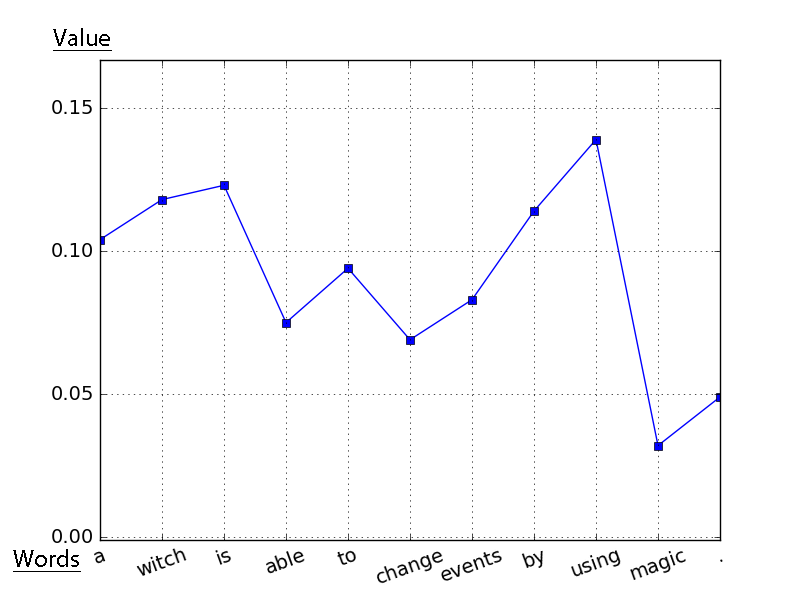
\includegraphics[width=.48\textwidth]{chapter4_experiments/images/sem-val1.png}
}
\subfigure[book - catalogues]{
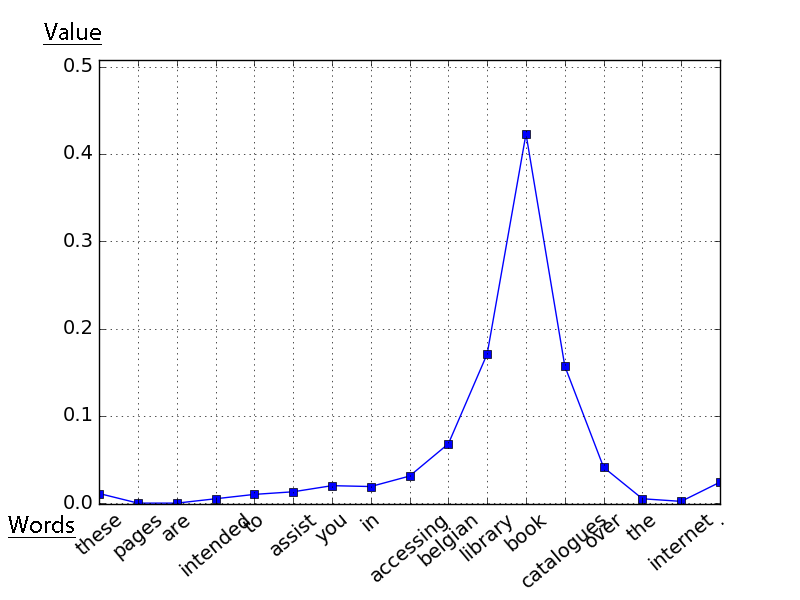
\includegraphics[width=.48\textwidth]{chapter4_experiments/images/sem-val2.png}
}
\subfigure[plant - storage unit]{
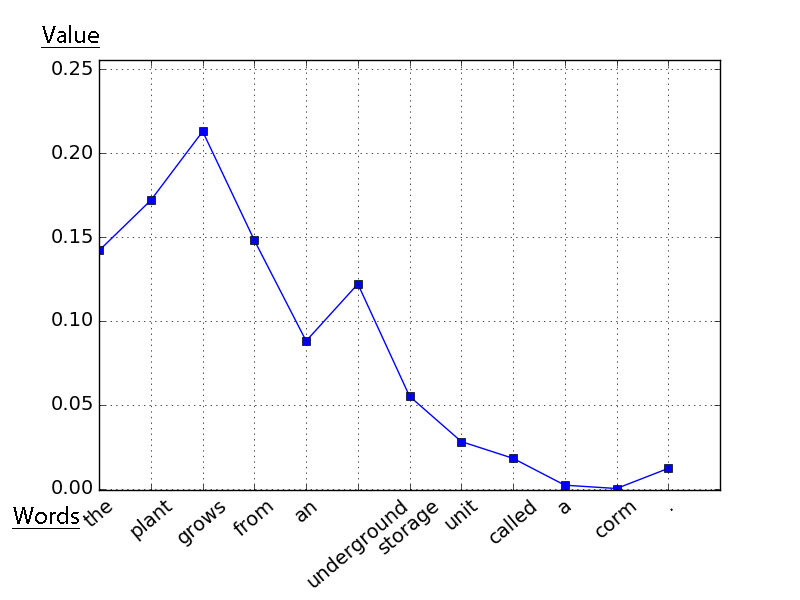
\includegraphics[width=.48\textwidth]{chapter4_experiments/images/sem-val3.png}
}
\caption[Semantic values, general domain supervised experiments]{Corresponding plots for three selected sentences from the test set of SemEval2010 for calculation of semantic values for words in the sentence.}
\label{fig:semantic-val}
\end{figure}

\paragraph{Scores distribution} This experiment is described in Subsection \ref{subs:score-distr}. It helps to look into the differences of scores given by the network to the relational classes.
The Figure \ref{fig:scores-distr} shows it for the same three examples, that were used for the 
experiment with semantic values. The first sentence is correctly classified and it can be seen, that all other scores are 
negative and only the correct class gives a comparatively large positive score. The second sentence 
distribution shows that network was hesitating between two acceptable classes and thus it 
got two small, but positive scores for both of them. The third sentence was recognised as 
''Other'',
 thus all the scores have to be negative. But two classes got very small negative scores, that are 
 correct class ''Entity-Origin'' and very close to the context of the sentence ''Product-Producer''.

\begin{figure}[H]
\centering
\subfigure[InstrumentAgency]{
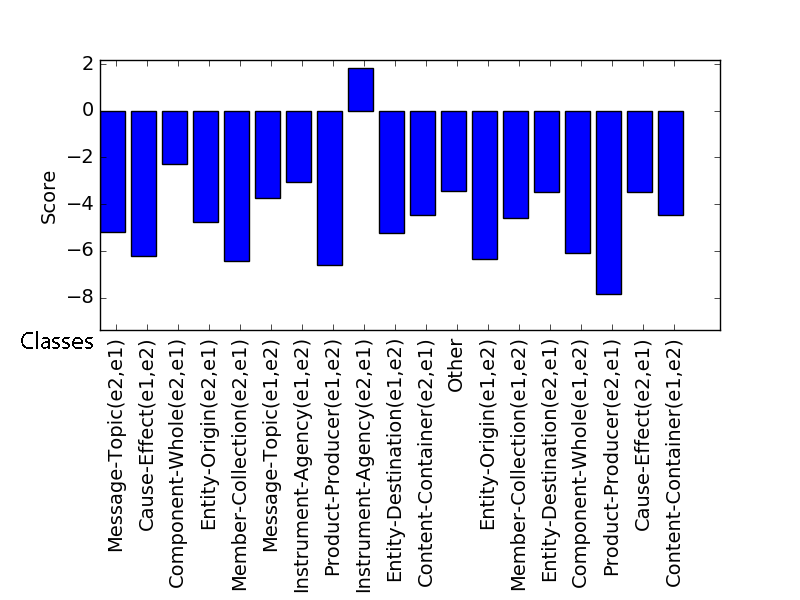
\includegraphics[width=.47\textwidth]{chapter4_experiments/images/scores1.png}
}
\subfigure[ComponentWhole]{
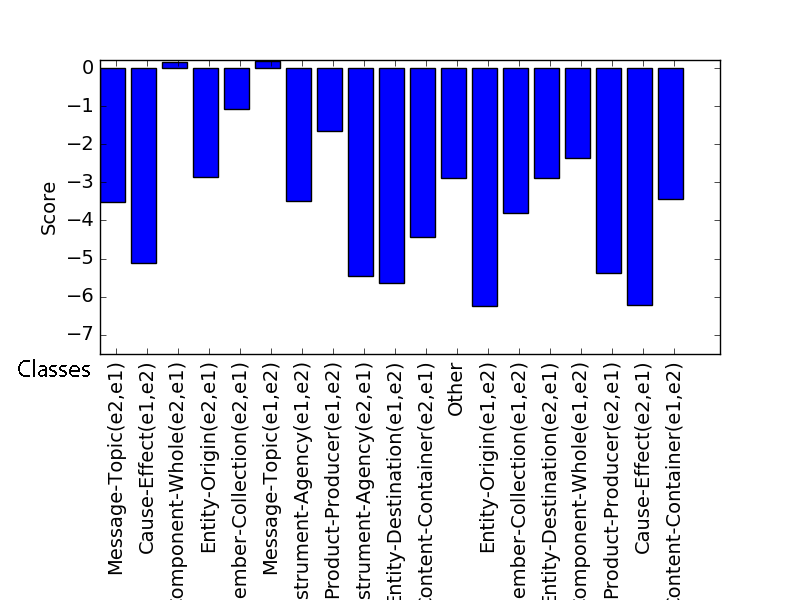
\includegraphics[width=.47\textwidth]{chapter4_experiments/images/scores2.png}
}
\subfigure[EntityOrigin]{
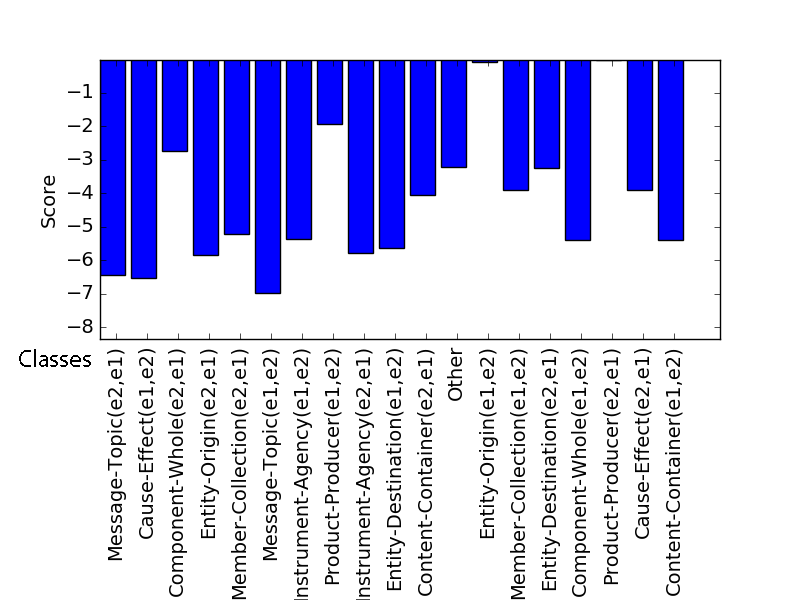
\includegraphics[width=.47\textwidth]{chapter4_experiments/images/scores3.png}
}
\caption[Scores distributions, general domain supervised experiments]{Scores distributions of relational classes for three chosen sentences from the test set of SemEval2010.}
\label{fig:scores-distr}
\end{figure}

